\clearpage
\section{Algorithm and Code Explanation}

\subsection{Data Pretreatment}
We use sklearn, a popular third-party package for machine learning, as well as numpy tools to help solving these problems. We are provided with four data files\footnote{The data that we use is kindly offered by Professor Chen. It can be downloaded by:\\ https://pan.baidu.com/s/1AfZKtPzbjoFSL67KzldD8A \quad Password: rtx0} in npy format: test\_data, test\_label, train\_data and train\_label. Among these test\_data and train\_data are sets of 310 features and have the following format after loading into numpy array:

\begin{center}
feature1 feature2 feature3 ...feature310 (of data1)\\
feature1 feature2 feature3 ...feature310 (of data2)\\
......\\
feature1 feature2 feature3 ...feature310 (of datan)\\
\end{center}


Test\_label and train\_label are the label sets corresponding to the two feature sets respectively, and are one-dimensional arrays when loaded into numpy array. This is a three-class problem and there are three kinds of labels: 1,0 and -1.


In order to facilitate the later data selection and processing, we disrupt the order of both the training set and test set (note that same random seeds should be used for feature sets and label sets to ensure the correspondence does not change). Considering the similar value range of each feature, we do not use data normalization in the pretreatment.
\subsection{Problem 1}
The first problem is to solve the three-class classification problem in the given dataset using SVM Classifiers and the one-vs-rest strategy. The principle of classification has been explained in Introduction. We use sklearn's function SVC(decision\_function\_shape='ovr') to train the one-vs-rest SVM model and solve this problem directly.

\subsection{Problem 2}
The second problem is to solve the three-class classification problem using min-max Module SVM and part-vs-part task decomposition method. Explanation of the our algorithm is given below. At the end of this section we also draw a process diagram to make the whole process intuitive. Note that the following algorithm is based on the paper\cite{lu2000emergence} \cite{王开安2005最小最大模块化支持向量机及其在文本分类中的应用}.
\subsubsection{Training Feature Set are Divided by Labels}
According to the corresponding labels, the training feature set is divided into three small feature sets: set1,set2 and set3, with corresponding labels 1, 0 and -1 respectively. For easy indexing, three small feature sets are placed in a list called sets.
\subsubsection{Three-class Problem To Two-class Problems}
We divide this three-class problem into three two-class problems, which are two-class problem between set1 and set2, two-class problem between set2 and set3, and two-class problem between set1 and set3. Consider the label of one of the sets in each pair (which in the code we call "positive set") as 1, and the label of the other set (which in the code we call "negative set") as -1. That is:

$$X^{+} =\left \{ \left ( x_{i}^{+} ,+1  \right )  \right \} _{i=1}^{l^{+} }$$
$$X^{-} =\left \{ \left ( x_{i}^{-} ,-1  \right )  \right \} _{i=1}^{l^{-} }$$


$l^{+}$ is the number of samples of positive set , $l^{-}$ is the number of samples of negative set. $X^{+}$ is the"positive class", $X^{-}$ is"negative class".


\subsubsection{Further Decomposition of Positive Set and Negative Set}
Further decompose positive set and negative set. The positive set is decomposed into $N^{+}$ subsets, and the negative set is decomposed into $N^{-}$ subsets. $N^{+}$ and $N^{-}$ are determined by the number of samples $l^{+}$ and $l^{-}$ and the preset parameters $\rho$. Their relationship is as follows:
$$N^{r} =\left [ \frac{l^{r} }{\rho }  \right ] ,r\in \left \{ +,- \right \} $$
where $\left [ x \right ]$ means to round x.


There are many different strategies to split the positive set and the negative set. We split them using the numpy function numpy.array.split(). The effect of this function is to decompose the original set into mutually disjoint subsets, and the number of samples of all the subsets differ from each other by no more than 1. For example, for a set of 10 samples, the number of samples of the subsets using function numpy.array.split() is 3,3,2,2. Thus, it is very simple to split the sets using function numpy.array.split(), and the result is very uniform.


The principle of the numpy.array.split() function can be expressed as follows:
$$
l_{i}^{r}=\left\{\begin{array}{l}
\left\lfloor\frac{l^{r}}{N^{r}}\right\rfloor \quad i>\left(l^{r} \bmod N^{r}\right) \\
\left\lfloor\frac{l^{r}}{N^{r}}\right\rfloor+1 \quad \text { others }
\end{array}, r \in\{+,-\}\right.
$$

\subsubsection{Sub-two-class Problems and Max-Mins Strategy}
After the positive set is decomposed into $N^{+}$ subsets and the negative set is decomposed into $N^{-}$ subsets, the original two-class problem becomes  $N^{+}\times N^{-}$ sub-two-class problems. Then set T of size $N^{+}\times N^{-}$ can be obtained. The training set of sub-two-class problem $T_{i,j}$ (including feature set and label set) can be intuitively represented by Figure \ref{fig:Training set of sub-two-class problem T_{i,j}}, where $1\le i\le N^{+} ,1\le j\le N^{-}$.

\begin{figure}[h!]
    \centering
    \includegraphics[scale=0.5]{figures/Training set of sub-two-class problem T_{i,j}.png}
    \caption{Training set of sub-two-class problem $T_{i,j}$}
    \label{fig:Training set of sub-two-class problem T_{i,j}}
\end{figure}

For each sub-two-class problem, a small SVM is trained by using sklearn's SVC module. Then the set (matrix) of small vector machines of size $N^{+}\times N^{-}$ can be obtained,  which we call set M.
If the feature set of test set is input into M, the predict label set is obtained, which we call set Predict\_val. The maximum and minimum strategy are adopted for Predict\_val, that is, taking the minimum value of each row of Predict\_val and then taking the maximum value of the result. Then the predict label of the original two-class problem can be obtained. The plus or minus of  this label determines the result of the original two-class problem.

\subsubsection{Vote and Accuracy}
Among set1, set2 and set3, the set with the most votes is the final predict set of the feature set for the test data.


The accuracy can be calculated by comparing the final predict set with the set to which the feature set originally belongs.
\subsubsection{Process Diagram}
The process diagram of the whole process is shown in Figure \ref{fig:Process diagram of problem 2}.
\begin{figure}[h!]
    \centering
    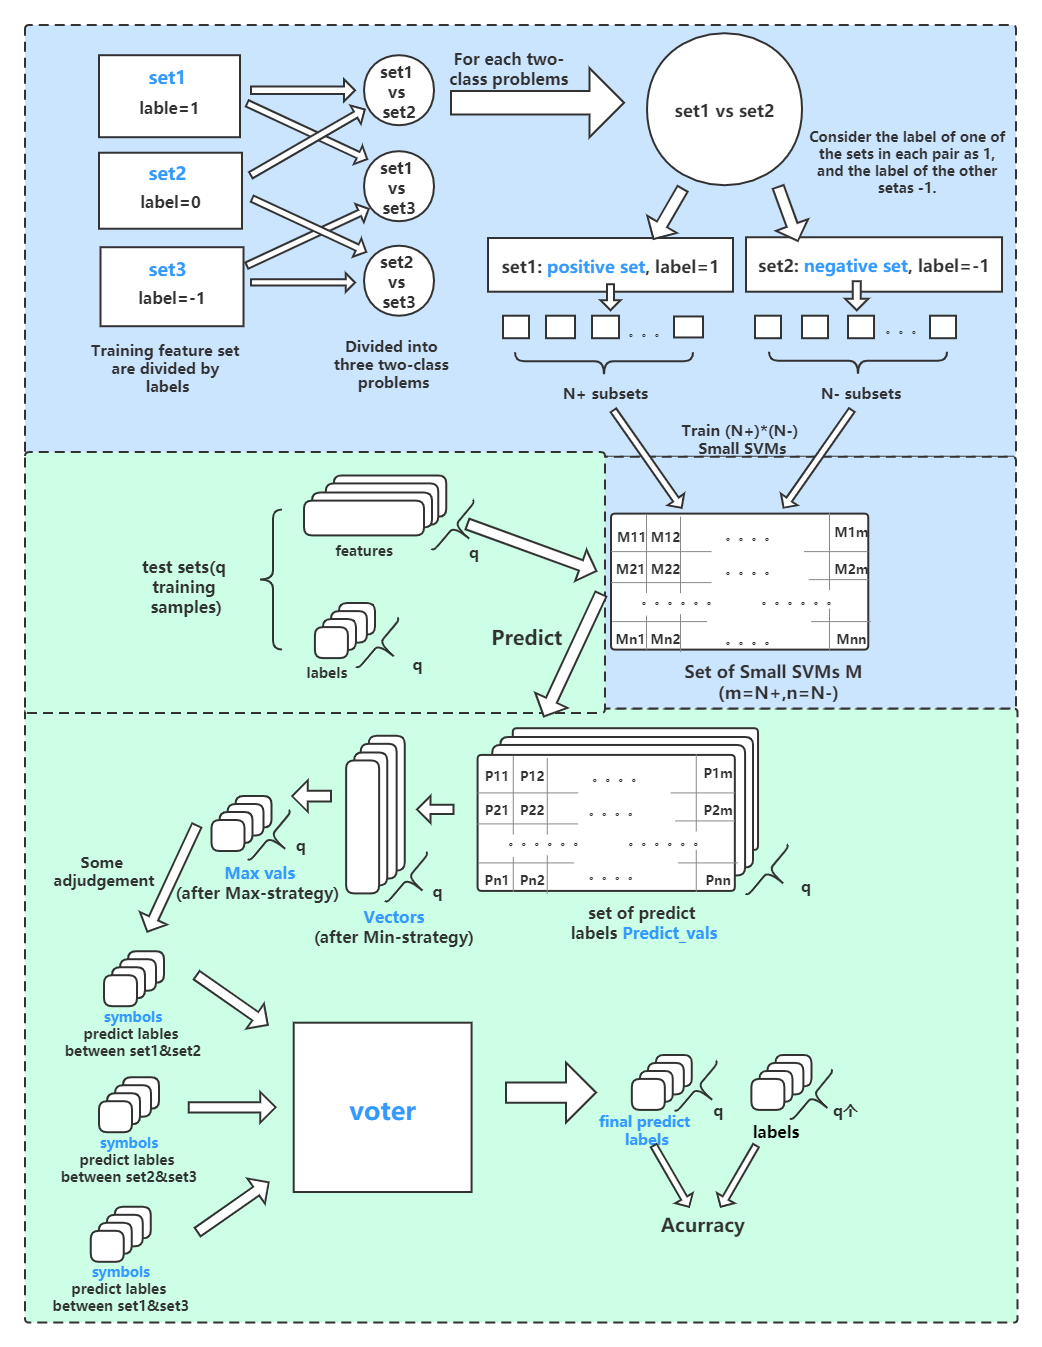
\includegraphics[width=\textwidth]{figures/Process diagram of problem 2.png}
    \caption{Process diagram of problem 2}
    \label{fig:Process diagram of problem 2}
    Notes: Words in blue colour are names of variables or matrixs used in the code;
Blue background means training phase and green background means testing phase
\end{figure}



